\documentclass[10pt]{article}  

%%%%%%%% PREÁMBULO %%%%%%%%%%%%
\title{Lógica difusa aplicada a las estructuras de hormigón}
\usepackage[spanish]{babel} %Indica que escribiermos en español
\usepackage[utf8]{inputenc} %Indica qué codificación se está usando ISO-8859-1(latin1)  o utf8  
\usepackage{amsmath} % Comandos extras para matemáticas (cajas para ecuaciones,
% etc)
\usepackage{amssymb} % Simbolos matematicos (por lo tanto)
\usepackage{graphicx} % Incluir imágenes en LaTeX
\usepackage{color} % Para colorear texto
\usepackage{subfigure} % subfiguras
\usepackage{float} %Podemos usar el especificador [H] en las figuras para que se
% queden donde queramos
\usepackage{capt-of} % Permite usar etiquetas fuera de elementos flotantes
% (etiquetas de figuras)
\usepackage{sidecap} % Para poner el texto de las imágenes al lado
	\sidecaptionvpos{figure}{c} % Para que el texto se alinie al centro vertical
\usepackage{caption} % Para poder quitar numeracion de figuras
\usepackage{commath} % funcionalidades extras para diferenciales, integrales,
% etc (\od, \dif, etc)
\usepackage{cancel} % para cancelar expresiones (\cancelto{0}{x})
 
\usepackage{anysize} 					% Para personalizar el ancho de  los márgenes
\marginsize{2cm}{2cm}{2cm}{2cm} % Izquierda, derecha, arriba, abajo

\usepackage{appendix}
\renewcommand{\appendixname}{Apéndices}
\renewcommand{\appendixtocname}{Apéndices}
\renewcommand{\appendixpagename}{Apéndices} 

% Para que las referencias sean hipervínculos a las figuras o ecuaciones y
% aparezcan en color
\usepackage[colorlinks=true,plainpages=true,citecolor=blue,linkcolor=blue]{hyperref}
%\usepackage{hyperref} 
% Para agregar encabezado y pie de página
\usepackage{fancyhdr} 
\pagestyle{fancy}
\fancyhf{}
\fancyhead[L]{\footnotesize INTELIGENCIA COMPUTACIONAL} %encabezado izquierda
\fancyhead[R]{\footnotesize }   % dereecha
\fancyfoot[R]{\footnotesize }  % Pie derecha
\fancyfoot[C]{\thepage}  % centro
\fancyfoot[L]{\footnotesize Master en Ingeniería Informática}  %izquierda
\renewcommand{\footrulewidth}{0.4pt}


\usepackage{listings} % Para usar código fuente
\definecolor{dkgreen}{rgb}{0,0.6,0} % Definimos colores para usar en el código
\definecolor{gray}{rgb}{0.5,0.5,0.5} 
% configuración para el lenguaje que queramos utilizar
\lstset{language=Matlab,
   keywords={break,case,catch,continue,else,elseif,end,for,function,
      global,if,otherwise,persistent,return,switch,try,while},
   basicstyle=\ttfamily,
   keywordstyle=\color{blue},
   commentstyle=\color{red},
   stringstyle=\color{dkgreen},
   numbers=left,
   numberstyle=\tiny\color{gray},
   stepnumber=1,
   numbersep=10pt,
   backgroundcolor=\color{white},
   tabsize=4,
   showspaces=false,
   showstringspaces=false}

\newcommand{\sen}{\operatorname{\sen}}	% Definimos el comando \sen para el seno
%en español

\title{Lógica difusa empleada al uso de estructuras de hormigón}

%%%%%%%% TERMINA PREÁMBULO %%%%%%%%%%%%

\begin{document}

%%%%%%%%%%%%%%%%%%%%%%%%%%%%%%%%%% PORTADA %%%%%%%%%%%%%%%%%%%%%%%%%%%%%%%%%%%%%%%%%%%%
																					%%%
\begin{center}																		%%%
\newcommand{\HRule}{\rule{\linewidth}{0.5mm}}									%%%\left
 																					%%%
\begin{minipage}{0.48\textwidth} \begin{flushleft}

\includegraphics[scale = 0.35]{Imagenes/logougr.eps}
\end{flushleft}\end{minipage}
\begin{minipage}{0.48\textwidth} \begin{flushright}

\includegraphics[scale = 0.63]{Imagenes/decsailogo.eps}
\end{flushright}\end{minipage}

													 								%%%
\vspace*{0.5cm}								%%%
																					%%%	
\textsc{\huge Universisdad de Granada}\\[1.5cm]	

%\textsc{\LARGE Unidad Profesional Interdisciplinaria en Ingenier\'ia y				%%%
%Tecnolog\'ias Avanzadas}\\[1.5cm]													%%%

\begin{minipage}{0.9\textwidth} 
\begin{center}																					%%%
\textsc{\LARGE Aplicación de la Lógica Difusa}
\end{center}
\end{minipage}\\[0.5cm]
%%%
    																				%%%
 			\vspace*{1cm}																		%%%
																					%%%
\HRule \\[0.4cm]																	%%%
{ \huge \bfseries Lógica Difusa Aplciada a las Estructuras de Hormigón}\\[0.4cm]	%%%
 																					%%%
\HRule \\[1.5cm]																	%%%
 																				%%%
																					%%%
\begin{minipage}{0.46\textwidth}													%%%
\begin{flushleft} \large															%%%
\emph{Autores:}\\	
Manuel Jesús García Manday
\\Mario Ortega Aguayo
%%%
			%\vspace*{2cm}	
            													%%%
										 						%%%
\end{flushleft}																		%%%
\end{minipage}		
																%%%
\begin{minipage}{0.52\textwidth}		
\vspace{-0.6cm}											%%%
\begin{flushright} \large															%%%
													%%%
\end{flushright}																	%%%
\end{minipage}	
\vspace*{1cm}
%\begin{flushleft}
 	
%\end{flushleft}
%%%
 		\flushleft{\textbf{\Large Master en  Ingeniería Informática}	}\\																		%%%
\vspace{2cm} 																				
\begin{center}																					
{\large \today}																	%%%
 			\end{center}												  						
\end{center}							 											
																					
\newpage																		
%%%%%%%%%%%%%%%%%%%% TERMINA PORTADA %%%%%%%%%%%%%%%%%%%%%%%%%%%%%%%%

\tableofcontents 

\newpage

\section{Resumen.}



El artículo hace una reflexión sobre las alternativas que existen para las estructuras de hormigón, in situ y prefabricadas, profundizando en métodos multicriterio(*) como ayuda a la toma de decisiones. Presenta un sistema de ayuda a la toma de decisiones basado en matemática difusa, que lo que hace es considerar el valor de cada alternativa contemplando el riesgo inherente. Lo ilustra mediante un ejemplo que puede resolverse a través de prefabricación  o in situ, llegando a dos conclusiones principales: la bondad de la herramienta presentada y como la solución prefabricada, en este caso, aporta mayor valor. Concluye también indicando que todo buen gestor debe plantearse su toma de decisiones desde los inicios de cualquier proyecto, empleando herramientas con la presentada.



\section{Introducción.} 

Las soluciones prefabricadas, tanto en obra civil como en edificación, son cada vez más utilizadas frente a las soluciones in situ.\\ 

Mediante las técnicas multicriterio se puede cuantificar las características de una alternativa para la toma de decisiones. Estas técnicas inicialmente se trataron de forma teórica en el ámbito de la economía y la gestión empresarial, pero el interés despertado en el ámbito de la construcción hizo que se desarrollaran diversos modelos  para la toma de decisión en diversos aspectos dentro de este marco como la contratación, la construcción y el diseño, estudio de alternativas y la resolución de conflictos. \\

La eficiencia de trabajos de construcción está correlacionada con la calidad de las tomas de decisión. Se necesita el apoyo en hechos y no en opiniones para decidir con fundamento; sin embargo, la evaluación de acciones que todavía no han ocurrido requieren el uso de metodologías que disminuyan el efecto de la subjetividad de los agentes en la perdida de calidad del proceso de toma de decisiones.\\

El problema de la toma de decisión adquiere un especial relevancia al plantearse el dilema entre la ejecución in situ y una posible solución prefabricada. La creciente demanda del sector de la construcción, especialmente motivada por los recientes cambios que ha experimentado la sociedad, hacen que intervengan cada vez más parámetros en la toma de decisión. A las variables tradicionales como son el coste, el plazo y la calidad, se añaden nuevos requisitos como la seguridad de los operarios, el respeto al medio ambiente o el ahorro de recursos naturales. \\

Es en este marco donde se propone la aplicación de un método de toma de decisiones denominado <<Integrated Decision System>> para la elección entre una solución u otra. Dicho método aporta una estructura de razonamiento que integra los diferentes aspectos mencionados en el párrafo anterior. A través de la lógica difusa incorporada en este método es posible obtener una evaluación flexible de las diversas alternativas, teniendo en cuenta que algunos parámetros serán de carácter cuantitativo (coste, plazo, variables físicas) y otros un valor mas intangible (aspectos estéticos, sociales, etc.).\\

El objetivo del sistema de toma de decisiones es conseguir un estudio mas riguroso de la decisión, de manera que sea más objetiva integrando las diversas vertientes y las múltiples variables del problema.\\


El empleo de la lógica difusa frente a otros métodos se fundamenta en su capacidad para modelizar la ambigüedad.\\

Este trabajo tiene por objeto presentar el modelo multicriterio IDS y mostrar un ejemplo de aplicación para la construcción de pasos inferiores, analizando soluciones in situ y prefabricadas. \\

\section{Solución prefabricada o in situ: cuando sólo una alternativa es óptima.} 

La construcción es uno de los sectores mas relevantes y que mas repercusión tiene en la calidad de vida de las personas. La rápida evolución que ha experimentado el conocimiento ha dado lugar a que se extiendan dos ámbitos de modo particular:

\begin{itemize}
	
	\item Las metodologías de apoyo a la toma de decisiones en la gestión de proyectos, desde las grandes a las pequeñas decisiones.
	
	\item Las posibilidades de los sistemas prefabricados para dar soluciones de alta eficiencia en la confección de estructuras desde puntos de vista muy diversos (económico, temporal, funcional, social y medioambiental).

\end{itemize}

A modo de ejemplo ilustrativo, la Figura 1 presenta las medidas en función del grado de satisfacción bajo diversos puntos de vista de soluciones prefabricadas e in situ en Hong Kong para edificios residenciales y no residenciales. Cabe indicar que si bien esto no quiere decir que la alternativa prefabricada sea siempre la solución óptima.\\

\begin{figure}[H]
	\begin{center}
 		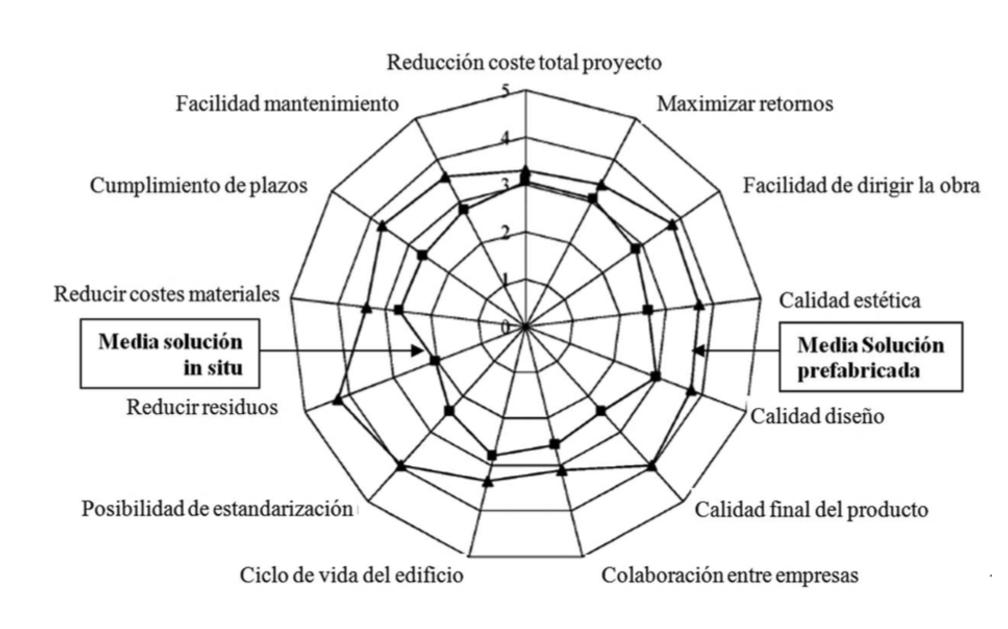
\includegraphics[width = 0.5\textwidth]{Imagenes/comparacion.eps}
 		\captionof{figure}{\label{fig:IPN}Comparación entre solución in situ y prefabricada.} 
	\end{center} 
\end{figure}

Como se puede ver en la gráfica de la Figura 1 para la situación particular de este escenario, el grado de satisfacción para cada uno de los diferentes aspectos es siempre mayor en las soluciones prefabricadas que en las soluciones realizadas in situ.\\

	Diversos autores como Sacks, Jailon y Polat nos muestran la desigualdad que hay presente en las soluciones prefabricadas en algunas sociedades de las que se podrían esperar un resultado parecido al de la Figura 1 en los datos recogidos desde 1998 por este ultimo, donde  países como Finlandia indica un extremo del 56% de soluciones prefabricadas frente a un 6% en EEUU. Mientras que en países como Alemania y el Reino Unido oscilan entre el 25% y el 30%, la situación en España de soluciones prefabricadas alcanza la cifra del 20%. Cabe indicar que todo esto depende evidentemente del tipo de aplicación en el que se da la solución prefabricada.\\

	Pueden existir diferentes factores por los que se obtengan esas diferencias en los datos. Una razón que lo explique puede verse reflejada en las condiciones climáticas, ya que en países donde el frío es mas evidente la solución prefabricada sería una opción para muchos casos inevitable. \\
	
	Este mismo autor intenta explicar la razón del bajo uso de las soluciones prefabricadas en EEUU, eliminando inferencias del siguiente tipo:

\begin{itemize}
	
	\item No hay dificultades relevantes en la incompatibilidad de los productos por falta de estandarización, si es que eso puede ser una dificultad.
	
	\item Las cuestiones estéticas se satisfacen mediante el diseño.
	
	\item Los usuarios de edificios prefabricados manifiestan su satisfacción de modo inequívoco.
	
	\item El comportamiento sísmico de las estructuras prefabricadas no es diferente de las estructuras resueltas con hormigón in situ.  

\end{itemize}

Otro factor del bajo uso de las soluciones prefabricadas en lugares donde sería adecuado en el que dicho autor hace referencia es la falta de profesionales que puedan diseñar y administrar la construcción con elementos prefabricados. Teniendo en cuenta incluso la repercusión negativa que diversos errores de diseño o concepción hayan podido incidir en la cultura colectiva.\\

	El momento en el que se decide cuando optar por una solución prefabricada es otro aspecto a tener en cuenta, ya que si el cambio se produce a mitad de un proyecto que inicialmente estaba diseñado para utilizar una solución in situ este se vería seriamente condicionado, por lo que ese tipo de decisiones es mejor tomarlas en las fases más temprana del diseño del proyecto.\\

	Es razonable pensar en incrementar la presencia de los métodos de análisis multicriterio para así reducir los riesgos de equivocarse en la toma de decisiones. Es en este contexto donde se sitúa en sistema integrado de decisiones (IDS).\\
	
	
\section{La herramienta de análisis: el sistema IDS.}

El sistema IDS se estructura en tres elementos principales: el concepto de valor y su modo de medición o evaluación, el concepto de riesgo y su tratamiento matemático y un proceso meteorológico denominado ACE (Análisis, Creatividad y Evaluación), donde se integran los dos elementos mencionados anteriormente.


\subsection{El valor. Concepto y medición.}

En el marco del desarrollo de un proyecto de construcción, el valor de una alternativa se define como el grado de satisfacción que produce. Se mide como la respuesta a los requerimientos del proyecto, considerando diversos planos como el económico, temporal, funcional, social y medioambiental.\\

	El valor es medido a través de una función, v(x), definida entre el rango 1 y -1, y que representa el grado de satisfacción que produce un parámetro de respuesta respecto a un cierto requerimiento, siendo 1 máxima satisfacción y -1 mínima satisfacción.\\

	Las funciones de valor de los diferentes requerimientos son integradas mediante un árbol de requerimientos, donde se pondera la importancia de cada uno de ellos y sus relaciones correspondientes. El cálculo del valor global de la alternativa se realiza con el despliegue de dicho árbol como se muestran en las siguiente expresiones:
	
\begin{figure}[H]
	\begin{center}
 		
\includegraphics[width = 0.5\textwidth]{Imagenes/expresion1.eps}
 		\captionof{figure}{\label{fig:IPN}} 
	\end{center} 
\end{figure}

\begin{figure}[H]
	\begin{center}
 		
\includegraphics[width = 0.5\textwidth]{Imagenes/expresion2.eps}
 		\captionof{figure}{\label{fig:IPN}} 
	\end{center} 
\end{figure}



\subsection{El riesgo. Concepto y tratamiento matemático.}

El concepto de riesgo se define como una incertidumbre por la falta de conocimiento en la previsión de los resultados relativos a los diversos requerimientos o por la posible variación de estos a causa de sucesos o agentes que tengan influencia sobre la realidad. Se distinguen dos tipos de riesgo, diferenciados por el tratamiento matemático que recibe cada uno de ellos:

\begin{itemize}

	\item riesgos especulativos: se define así a la incertidumbre que se asocia al conocimiento de un cierto resultado.
	
	\item riesgos puros: son los factores que pueden producir una variación en el valor del proyecto, produciendo una modificación en los parámetros de respuesta como el sobrecoste en el económico, el retraso en el temporal, etc.

\end{itemize}


El tratamiento de los riesgos especulativos se realiza mediante el uso de la matemática difusa. Más concretamente, lo que se hace es diseñar un elemento denominado “trapecio difuso” (Figura2) que constituye la base del planteamiento. Como se puede observar en la figura, dicho trapecio lo que hace es modelizar la incertidumbre que hay asociada al conocimiento de un cierto parámetro, como por ejemplo el coste o el tiempo de ejecución de una determinada obra. En dicho modelo se representa un intervalo más probable (b-c), y dos intervalos donde es menos probable que se encuadre el valor numérico del parámetro (a-b y c-d). El grado de probabilidad se modela mediante la función de pertenencia .\\

	La ventaja que tiene este planteamiento es que evita de este modo el uso de la probabilidad, algo que se antoja importante en un sector como el de la construcción donde los productos son singulares y no existe la respetabilidad necesaria para tener que plantear la evaluación de probabilidades.\\
	
	Del otro lado, la evaluación de los riesgos puros se realiza a través de un función de severidad, que es definida como la pérdida de valor que se produce del requerimiento debido al factor de riesgo. \\

	
	A partir de las funciones de severidad relativas a cada uno de los requerimientos a los que el riesgo puro afecta, se calcula la severidad total de modo de modo análogo al empleado para calcular riesgo especulativo, es decir, a través de la media ponderada según la estructura y pesos del árbol de requerimientos . Esa severidad debe substraerse del valor inicial, teniendo en cuenta los diversos riesgos puros que intervienen.\\


\subsection{El proceso ACE de toma de decisión.}

Es un proceso metodológico en el que se integran los elementos definidos anteriormente. En la siguiente tabla se recoge cual es su estructura.

\begin{figure}[H]
	\begin{center}
 		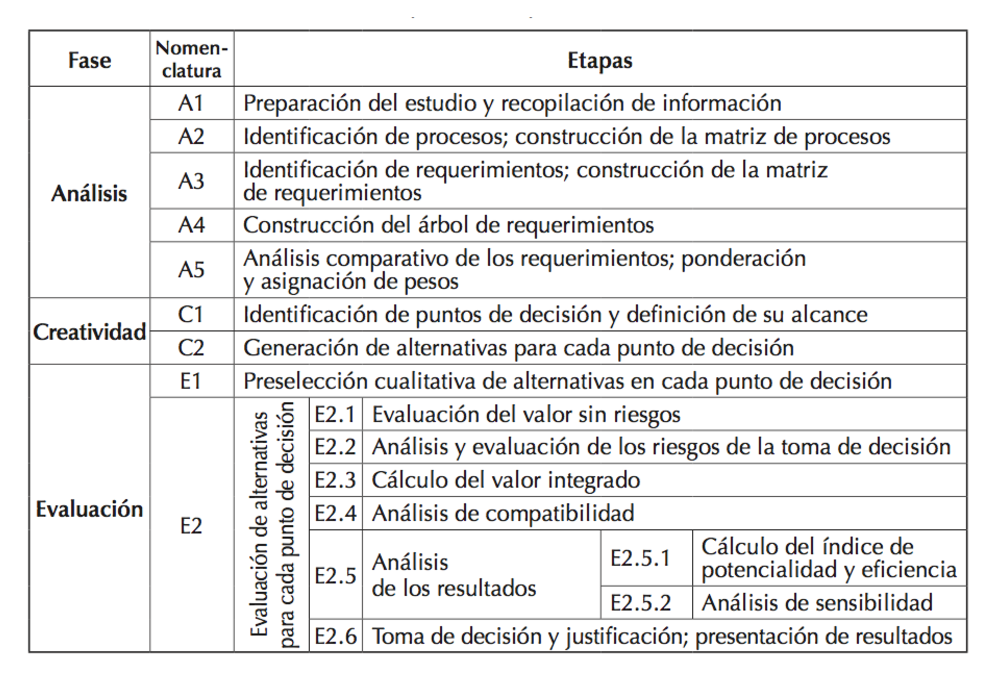
\includegraphics[width = 0.5\textwidth]{Imagenes/tabla1.eps}
 		\captionof{figure}{\label{fig:IPN}} 
	\end{center} 
\end{figure}

Este proceso es planteado como una estructura de razonamiento que puede ser aplciable tanto de manera cuantitativa mediante el uso de los modos de medición que se explicaron en los puntos anteriores, o de manera cualitativa a traves de la consideracion de los modelos conceptuales y la estructura que introduce.


\section{Caso de aplicación.}


\subsection{Características de las alternativas.}

Con el objetivo de concretar el planteamiento anterior se dispone a presentar un caso práctico, el cual se encuadra en las obras de una urbanización cercana a la costa y en una zona con elevado valor ecológico.\\

En este proyecto, se dispusieron tres obras de drenaje para permitir el flujo de pequeños torrentes hacia el mar por debajo de los viales. Para este hecho, se plantea la alternativa de sustituir la solución inicia del proyecto, en este caso la ejecución in situ, por una solución prefabricada y hastiales in situ.\\

En modo aclaratorio, el hastial o piñon es la zona arquitectónica o muro que va a servir a modo de aguante o sujeción al tejado o parte superior de la estructura. \\

Como podemos observar en la siguiente Figura 5, la cuál pertenece a la solución prefabricada, se va a componer realmente de unos hastiales in situ y una clave o arco prefabricado. Esto es debido a la falta de disponibilidad de elementos prefabricados en el mercado, por tanto, los hastiales se tendrían que ejecutar in situ al no existir moldes con esta altura de hastial para la Figura 6. Por otro lado, en caso de existir, la fabricación del mismo aumentaría considerablemente los plazos preestablecidos.

\begin{figure}[H]
	\begin{center}
 		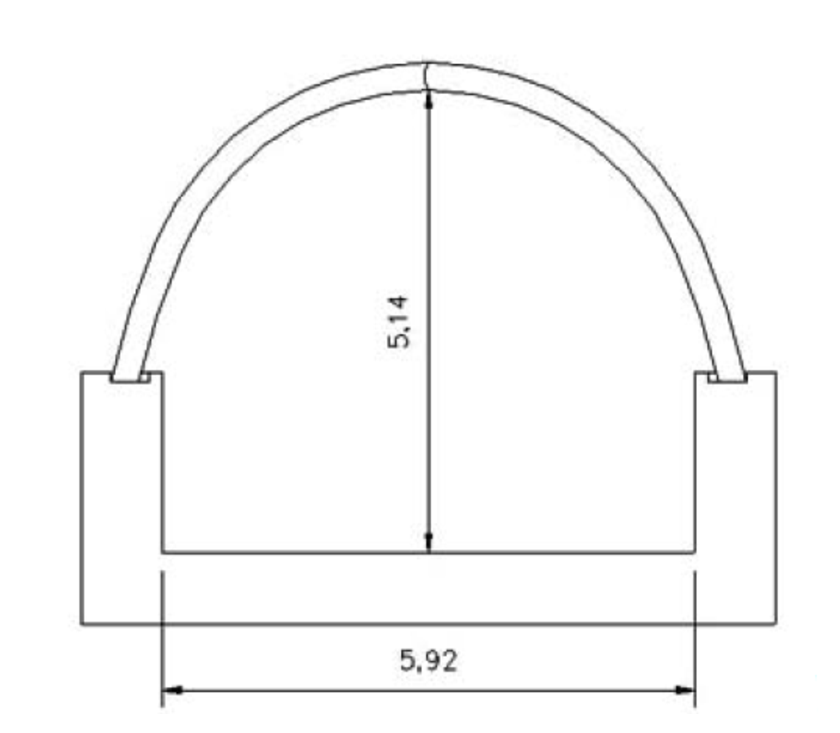
\includegraphics[width = 0.5\textwidth]{Imagenes/img1.eps}
 		\captionof{figure}{\label{fig:IPN}} 
	\end{center} 
\end{figure}

\begin{figure}[H]
	\begin{center}
 		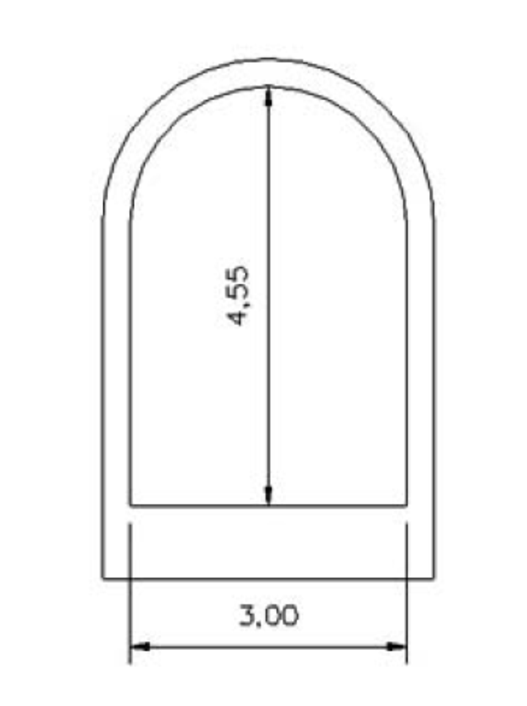
\includegraphics[width = 0.5\textwidth]{Imagenes/img2.eps}
 		\captionof{figure}{\label{fig:IPN}} 
	\end{center} 
\end{figure}

Con el objetivo de estudiar si la nueva solución prefabricada es más satisfactoria que la alternativa inicial in situ, se plantea la aplicación del sistema IDS, aplicando el proceso ACE, anteriormente descrito.

\subsection{Fase de análisis.}

En primer lugar, tenemos que identificar los requerimientos del proyecto, de forma que cada uno de los procesos incluidos en este proyecto se deben identificar con el esquema del proceso ACE. A partir de esta identificación, se construye el árbol de requerimientos, mostrado en la siguiente tabla y se lleva a cabo la ponderación relativa, según el método descrito por Ormazábal.\\

A continuación se muestra el árbol de requerimientos del proyecto estudiado. Cabe destacar que los requerimientos identificados hacen referencia al conjunto del proyecto, por tanto, la decisión finalmente considerada no afectará a muchos de ellos.\\

\begin{figure}[H]
	\begin{center}
 		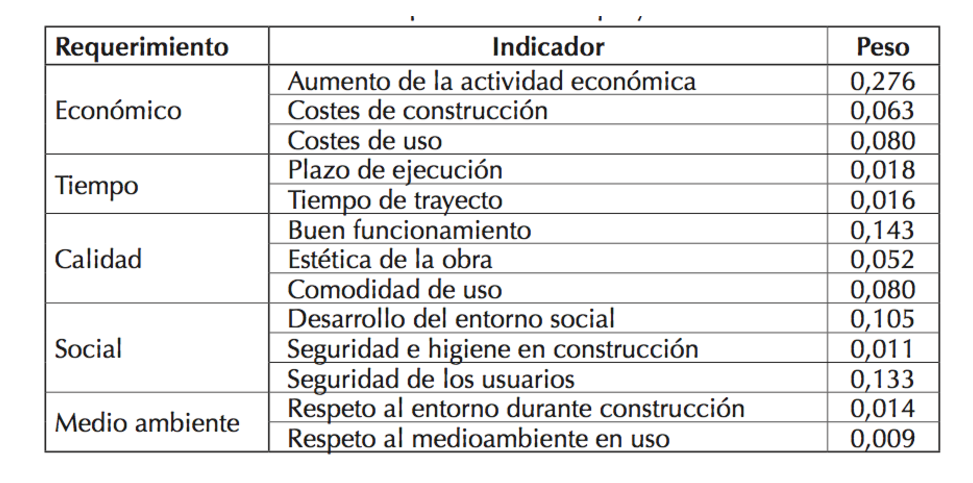
\includegraphics[width = 0.5\textwidth]{Imagenes/img3.eps}
 		\captionof{figure}{\label{fig:IPN}} 
	\end{center} 
\end{figure}

Para concluir esta fase, cabe indicar que existen requerimientos no contemplados en la figura anterior por considerarlos de menos importancia en el conjunto del proyecto. En este caso, tiene un papel crucial la creatividad del proceso ACE.

\subsection{Fase de evaluación.}

Una vez llegados a éste punto, el primer objetivo es identificar los parámetros de respuesta según lo indicado en el árbol de requerimientos, realizando un despliegue del mismo.\\

En el árbol de requerimientos desarrollado para este punto, el cual se muestra en la siguiente Figura 8, se puede observar que los parámetros de medición de la respuesta de las alternativas llevan asociados un peso, el cual corresponde a su grado de participación en el conjunto de la satisfacción del subrequerimiento correspondiente.

\begin{figure}[H]
	\begin{center}
 		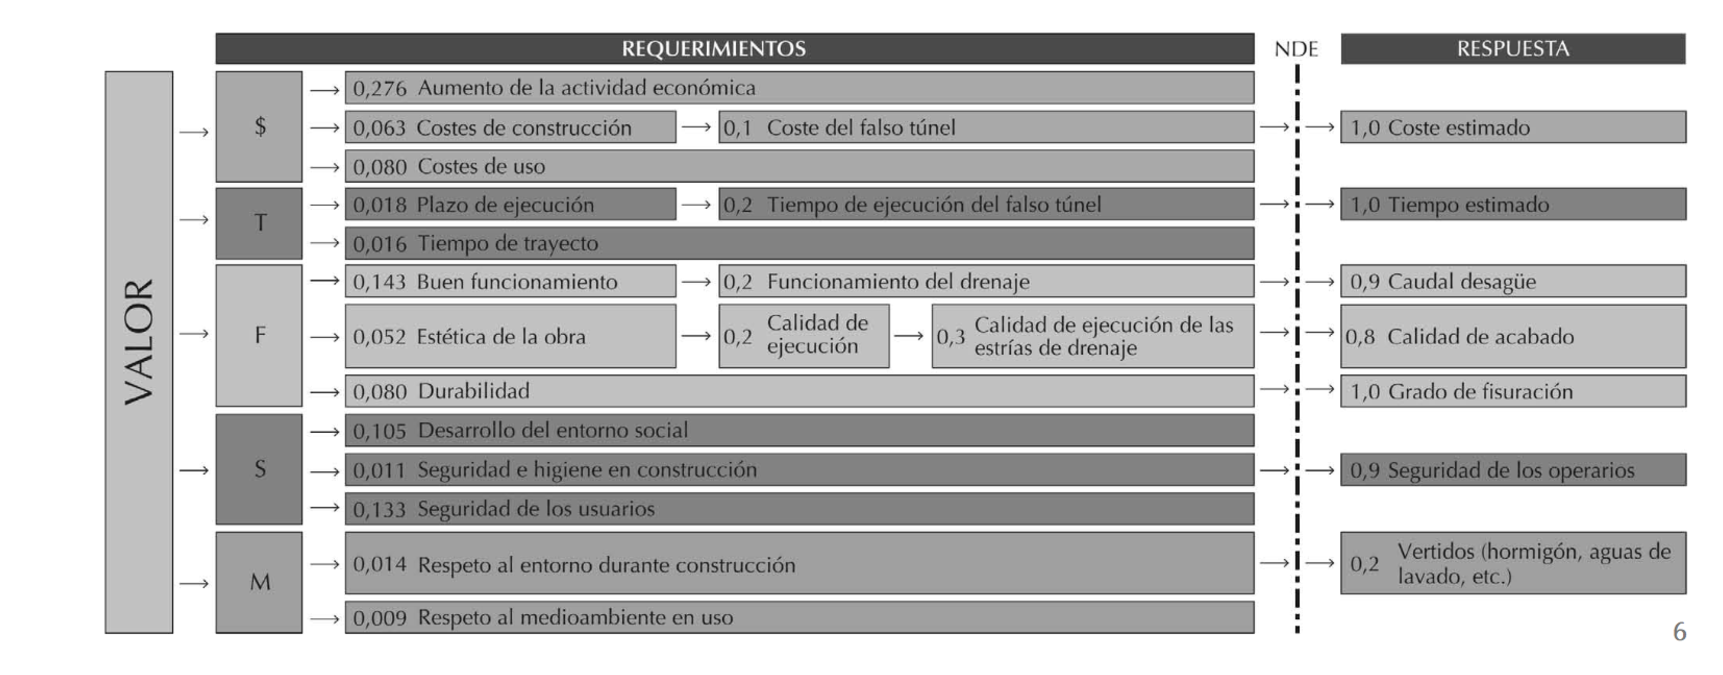
\includegraphics[width = 0.5\textwidth]{Imagenes/img4.eps}
 		\captionof{figure}{\label{fig:IPN}} 
	\end{center} 
\end{figure}

Respecto al coste económico, se deben considerar dos puntos importantes. En primer lugar, que el prefabricado incluye la necesidad del transporte, lo cuál puede aumentar de forma considerable el precio. Para este caso, dado el tamaño de las piezas, no tiene especial importancia. En cambio, el diseño del prefabricado es más optimizado al ejecutarse con un control más especializado, el cual no solo va a mejorar el propio diseño, sino que permite abaratar costes ya que se disminuyen factores de seguridad. Por otro lado, la asistencia técnica del proveedor del prefabricado podría ahorrar costes en cuanto a horas de ingeniería a la propia constructora, ya que esta asistencia puede aportar experiencia y asesoramiento técnico.\\

A continuación, se comenta el siguiente apartado, es decir, los plazos de la construcción. El hecho de utilizar prefabricado supone un ahorro severo de tiempo, ya que se evitan los inconvenientes de la construcción de hormigón a pie de obra. Esto supone tres claras ventajas.

\begin{itemize}

	\item Mejor acabado, ya que se realiza en condiciones menos adversas.
	
	\item Mayor durabilidad, asociada al nivel de fisuración, ya que el prefabricado soporta mayor resistencia a las soluciones in situ.

	\item Menos rugosidad del conducto de drenaje, lo cual implica una mayor capacidad de desaguar.

\end{itemize}

En relación al siguiente punto, relacionado con el plano social, se puede deducir que se evitan trabajos de andamio, lo cual aumenta la seguridad e higiene en el trabajo, disminuyendo el índice de siniestralidad. \\

Por último, en cuanto al medioambiente, se evitan vertidos de hormigón y se respetará el emplazamiento ecológico, importante en este estudio, ya que la construcción se sitúa cercana al mar.\\

Una vez terminada esta primera evaluación, se realiza una cuantificación más detallada, a través de funciones de valor de los requerimientos que hemos comentado anteriormente. Como podemos ver en la tabla siguiente, m y M representan los límites mínimo y máximo, y los valores que no tienen unidad se evalúan en un rango entre 1 y 10, que se asignará como resultado de expertos.

\begin{figure}[H]
	\begin{center}
 		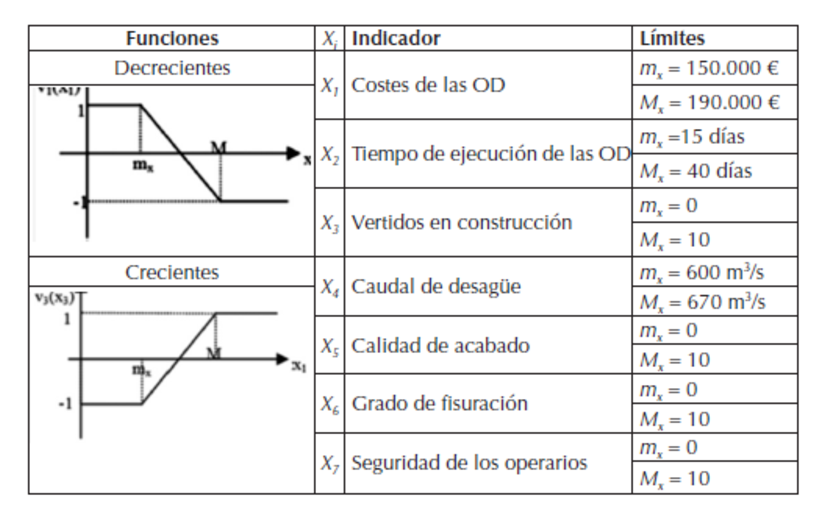
\includegraphics[width = 0.5\textwidth]{Imagenes/img5.eps}
 		\captionof{figure}{\label{fig:IPN}} 
	\end{center} 
\end{figure}

A partir de este despliegue del árbol se realiza la medición según el tratamiento difuso explicado en capítulos anteriores. Se debe destacar que, para este caso, se ha estimado mediante formas rectangulares en lugar de los trapecios dados. Por tanto, se toman a=b y c=d.

\begin{figure}[H]
	\begin{center}
 		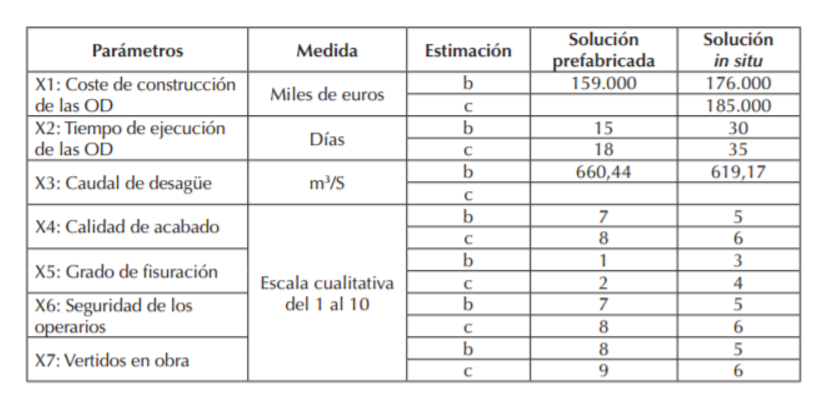
\includegraphics[width = 0.5\textwidth]{Imagenes/img6.eps}
 		\captionof{figure}{\label{fig:IPN}} 
	\end{center} 
\end{figure}

Como consecuencia de la obtención de las imágenes mediante la función v(x) se obtiene un resultado para cada alternativa. Como hemos indicado anteriormente, los resultados adoptarán una forma rectangular de cara a la obtención de la gráfica resultante, como podemos ver en la siguiente figura.

\begin{figure}[H]
	\begin{center}
 		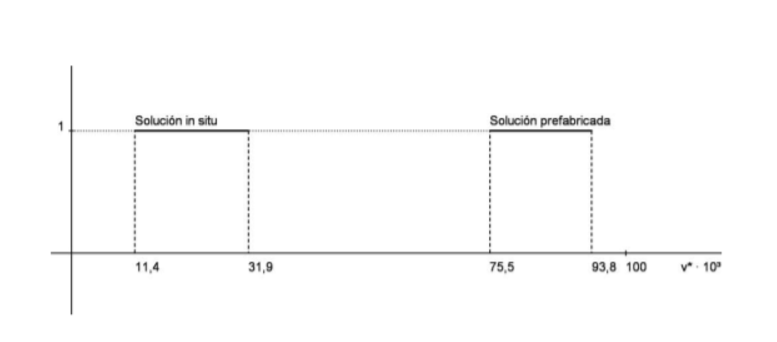
\includegraphics[width = 0.75\textwidth]{Imagenes/img7.eps}
 		\captionof{figure}{\label{fig:IPN}} 
	\end{center} 
\end{figure}

A continuación ,se va a realizar el proceso de evaluación de los valores añadiendo los riesgos.\\

En primer lugar, se realiza la identificación, análisis y evaluación de los riesgos para soluciones in situ y prefabricados.  Como se puede ver en la tabla siguiente, se toman los parámetros de evaluación de seguridad, para el posterior cálculo de la severidad.

\begin{figure}[H]
	\begin{center}
 		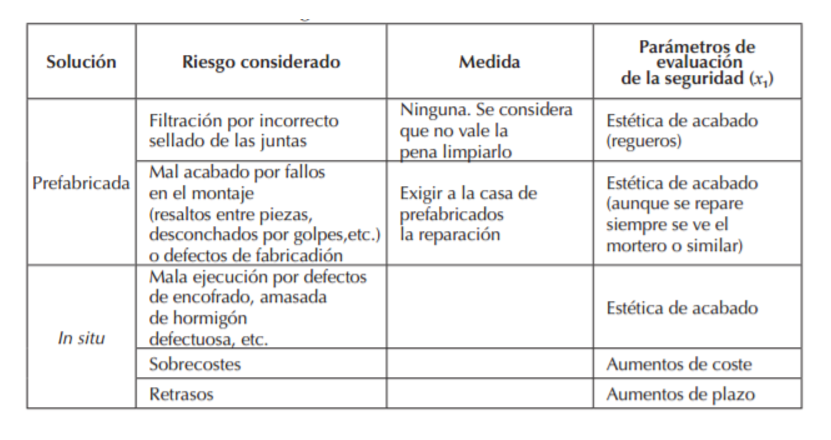
\includegraphics[width = 0.75\textwidth]{Imagenes/img8.eps}
 		\captionof{figure}{\label{fig:IPN}} 
	\end{center} 
\end{figure}

Una vez identificados los riesgos y los parámetros de evaluación de la seguridad, se realiza una nueva tabla donde se muestra el cálculo de la severidad una vez adoptadas estas medidas de respuesta. La probabilidad se calcula de forma subjetiva.\\

Estas pérdidas de calidad de acabado se miden a través de una puntuación en escala de 1 a 10. \\

Podemos ver dichos resultados en la siguiente figura.

\begin{figure}[H]
	\begin{center}
 		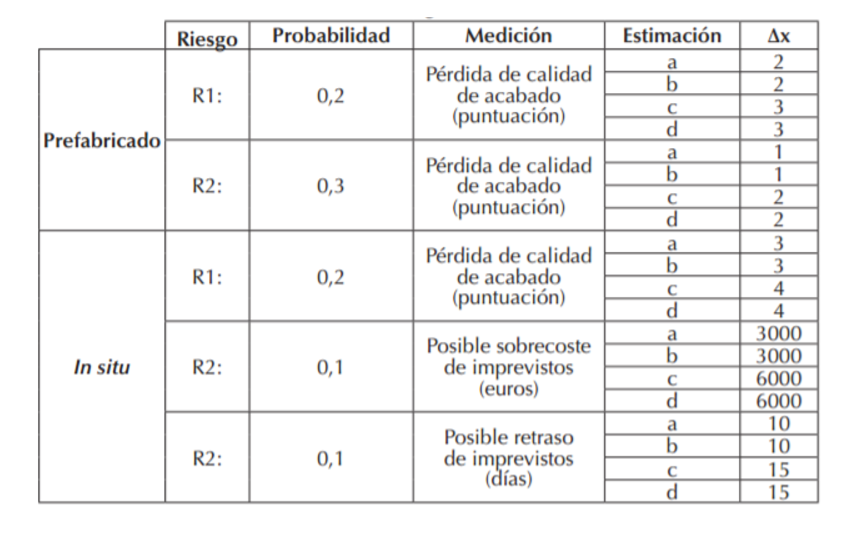
\includegraphics[width = 0.5\textwidth]{Imagenes/img9.eps}
 		\captionof{figure}{\label{fig:IPN}} 
	\end{center} 
\end{figure}

Desde el punto de vista del riesgo, el prefabricado aporta dos claras ventajas. En primer lugar, para la realización con hormigón in situ, la falta de mano de obra esp[ecializada implica que la impericia de los operarios pueda dar lugar a defectos que podrían desembocar en, como mínimo, peor estétiica. Por otro lado, no existe incertidumbre sobre los valores del coste y los plazos. El coste viene fijado por contraro mientras que el plazo no queda absolutamente asegurado, pero si cubierto por penalizaciones ocasionales. Para este último caso, si el proveedor es fiable este par;ametro podría ser despreciable. \\

A partir de estos resultados, se calcula la pérdida de valor que suponbe la posible existencia sde dichos riesgos, restando las severidades al valor calculado inicialmente. A continuación mostramos la tabla resultante.

\begin{figure}[H]
	\begin{center}
 		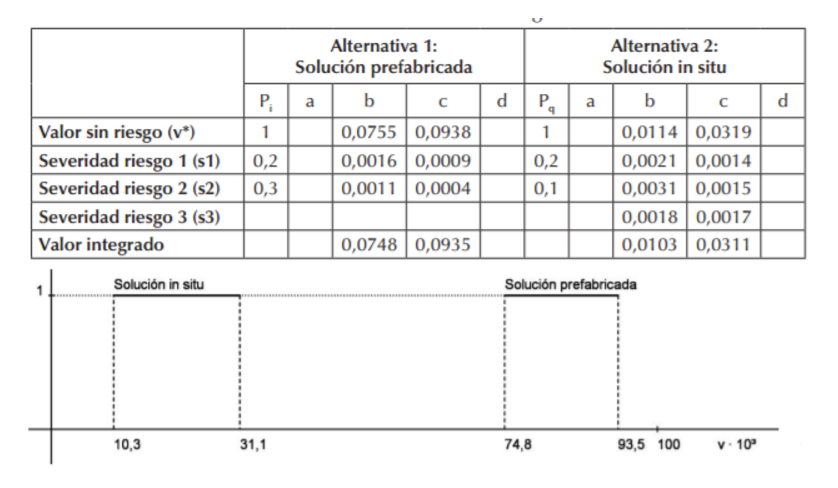
\includegraphics[width = 0.5\textwidth]{Imagenes/img10.eps}
 		\captionof{figure}{\label{fig:IPN}} 
	\end{center} 
\end{figure}

Al no observarse incompatibilidades en el análisis de resutlados, los resultados finales demuestran que el conjunto difuso asociado a la alternativa prefabricada obitnee valores más elevados que la opción in situ.. Por tanto, a la vista de los resultados, se escoje la opción prefabricada por estimarse que aporta un mayor valor al conjunto del proyecto.

\section{Conclusiones.}

El estudio realizado nos lleva a concluir con tres principales apartados a destacar.

\begin{itemize}

	\item El sistema integrado de decisiones (IDS) se ha mostrado eficiente para la resolución del problema planteado. Esta herramienta nos ha ayudado a solucionar los múltiples aspectos en  que se basa este proyecto, ya sea económico, temporal o social. El proceso de elección pasa por tres fases denominadas análisis, creatividad y evaluación.
	
	\item El sistema de decisiones para un gestor de proyecto debe ser una referencia, ya que la búsqueda de la solución óptima no debe de obviarse. Por tanto, cuando existan evidencias y recursos para ponderar dichas opciones, es más que recomendable la búsqueda de la solución optima aplicando el proceso aportado.
	
	\item La comparación de varios tipos de construcciones hace que podamos contrastar ambas soluciones, resultando favorable en este caso para el prefabricado.

\end{itemize}

%%%%%%% Bibliografía %%%%%%%%
\begin{thebibliography}{a}
\bibitem{pradery} \textsc{J. Armengou, A. Aguado, G. Ormazábal.},
\textit{An integrated decision-making methodology for the design of concrete structures.}
\bibitem{old} \textsc{H. Roche, C. Vejo.},
\textit{Análisis multicriterio en la toma de decisiones}
\end{thebibliography}




\end{document}